\bigbreak
\paragraph*{Što je SoftEther VPN?}
\hfill \smallbreak
\begin{wrapfigure}{r}{0.5\textwidth} 
     \centering
     
\includegraphics[width=0.5\textwidth]{SoftEther/SoftEtherLogo}
	\caption{Službeni logo SoftEther VPN-a}
\end{wrapfigure}

SoftEther VPN\cite{softether} besplatan je višeplatformski program otvorenog koda koji podržava korištenje različitih VPN protokola. Program je nastao 2013. godine kao akademski projekt na sveučilištu u Tsukubi i podržan je na različitim operacijskim sustavima kao što su Linux, FreeBSD, Mac, Solaris i Windows za koji je u ovom poglavlju prikazan postupak postavljanja i uporabe.
\smallbreak
Program SoftEther otvorenog je koda pa ga može bilo tko koristiti za vlastite ili komercijalne svrhe.\smallbreak
SoftEther VPN koristi HTTP preko SSL (Secure Sockets Layer)\cite{ssl}
protokola kako bi omogućio siguran prijenos kriptiranih podataka preko Interneta. Uz njega su podržani unutar programa i ostali poznatiji protokoli kao što su OpenVpn, IPsec, L2TP, ...\\
Unutar programa sve postavke detaljno su objašnjene i mogu se podesiti korištenjem grafičkog sučelja što ovaj program čini jednostavnim za uporabu.\\
\FloatBarrier
\smallbreak
Topologija koja se želi u ovom poglavlju ostvariti jest priključivanje korisnika udaljenoj mreži kao što je ilustrirano na slici \ref{fig:topologija-soft}. Korisnik će preko svojeg računala uspostaviti virtualni privatni tunel preko Interneta s računalom koje ima instaliran i konfiguriran SoftEther VPN server. Nakon povezivanja će korisnik pripadati logičkoj lokalnoj mreži servera.
\begin{figure}[h!]
	\centering
     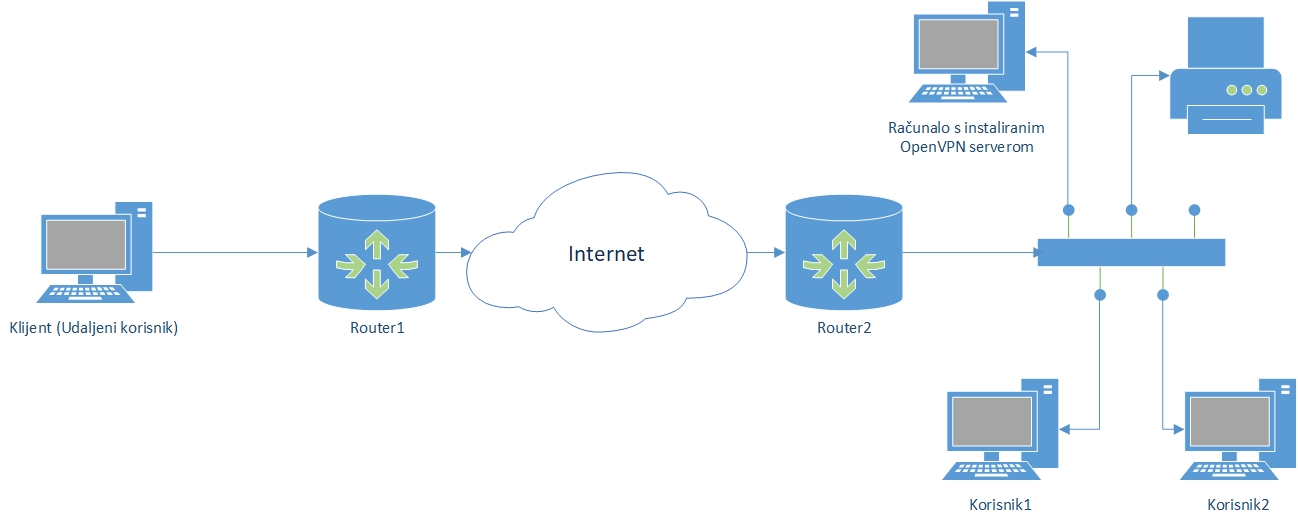
\includegraphics[width=0.9\textwidth]{SoftEther/topologija}
     \caption{VPN topologija}
     \label{fig:topologija-soft}
\end{figure}

\newpage
\paragraph*{Instalacija SoftEther servera}

\hfill \smallbreak
Za početak potrebno je preuzeti instalaciju VPN servera sa službene stranice SoftEthera:\\ \url{https://www.softether.org}
\begin{figure}[h!]
	\centering
     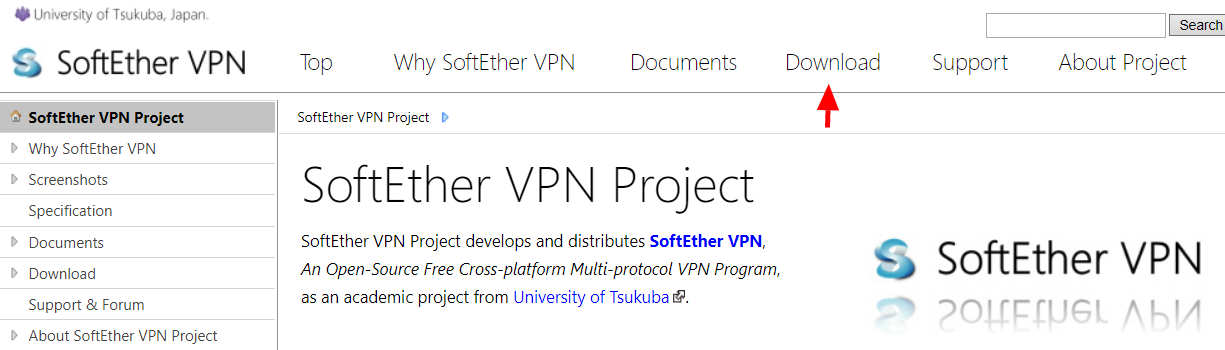
\includegraphics[width=0.7\textwidth]{SoftEther/korak1}
     \caption{Put do instalacije}
     \label{fig:link1-soft}
\end{figure}
\FloatBarrier
Odabirom ``Download'' iz izborne trake, što je prikazano na slici \ref{fig:link1-soft}., otvara se stranica s ponuđenim poveznicama za preuzimanje od kojih se odabire ona naglašena na slici \ref{fig:link2-soft}.
\begin{figure}[h!]
     \centering
     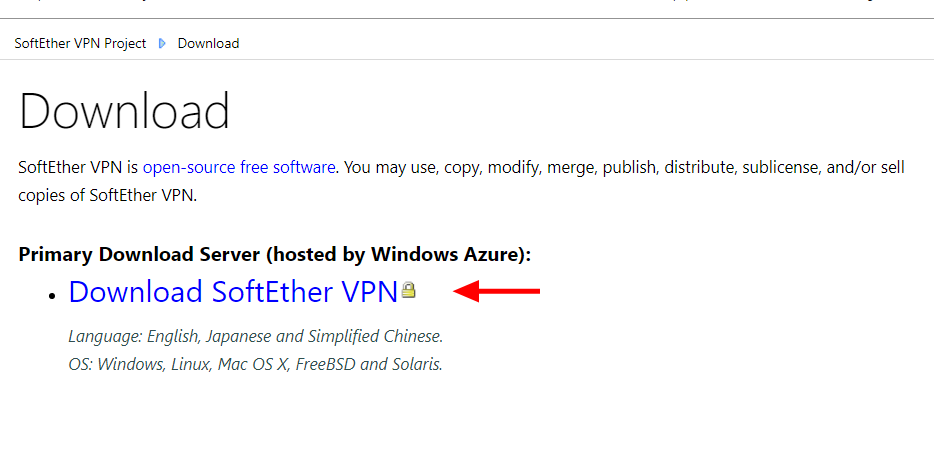
\includegraphics[width=0.55\textwidth]{SoftEther/korak2}
     \caption{Poveznica za odabir preuzimanja}
     \label{fig:link2-soft}
\end{figure}
\FloatBarrier
Sljedeći isječak(slika \ref{fig:link3-soft}.) prikazuje stranicu koja se otvori odabirom prve poveznice. Na stranici se nalaze izborni okviri u kojima je potrebno odabrati željeni program. Za preuzimanje VPN servera potrebno je odabrati postavke prikazane na sljedećem isječku te odabrati prvu poveznicu za početak preuzimanja.
\begin{figure}[h!]
     \centering
     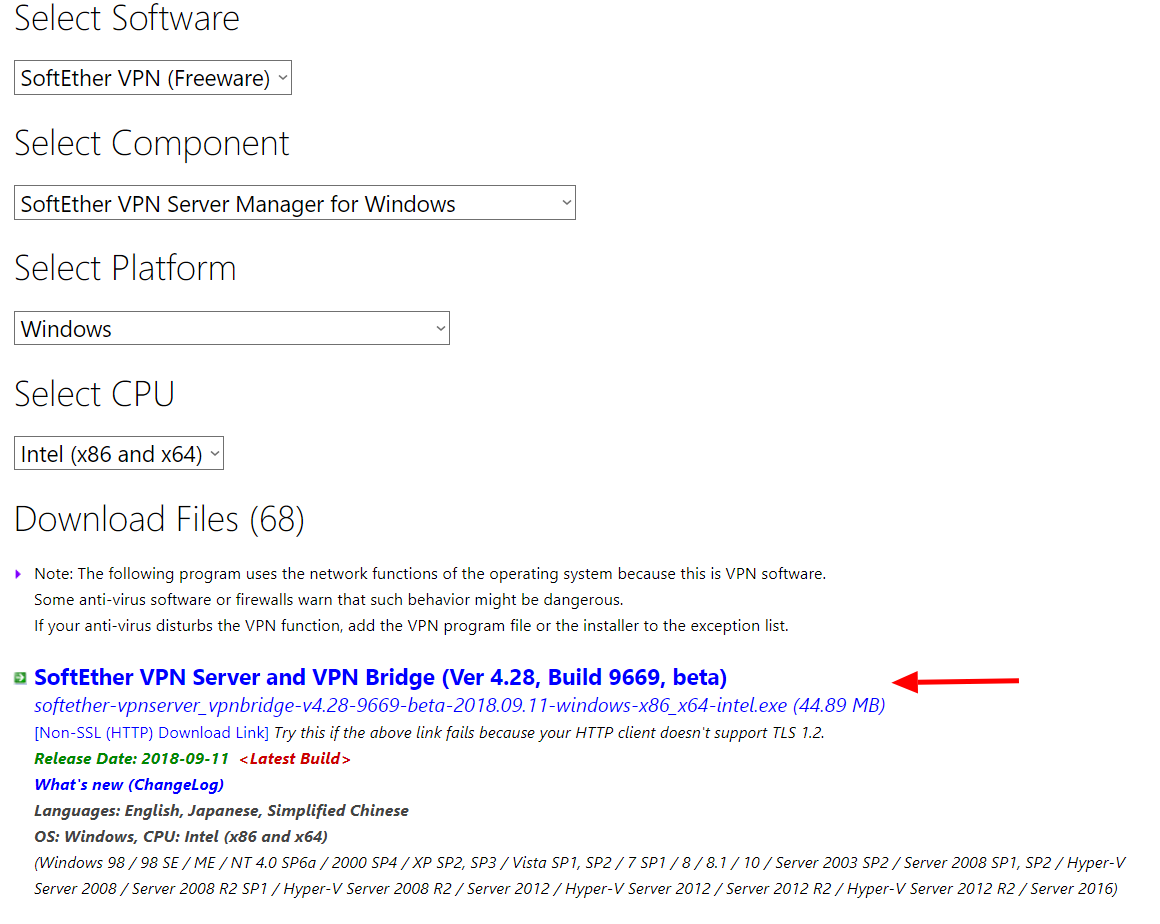
\includegraphics[width=0.6\textwidth]{SoftEther/korak6}
     \caption{Prikaz povaznice za preuzimanje}
     \label{fig:link3-soft}
\end{figure}
\FloatBarrier
Nakon preuzimanja i pokretanja instalacije otvara se prozor kao na slici \ref{fig:odabir-soft}. u kojemu se predlaže odabir prvog ponuđenog jer nudi potpunu instalaciju.
\begin{figure}[h!]
     \centering
     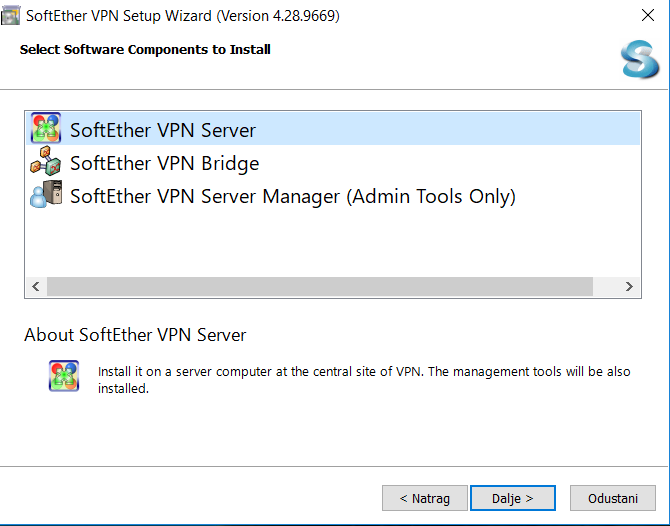
\includegraphics[width=0.6\textwidth]{SoftEther/korak7}
     \caption{Odabir servera}
     \label{fig:odabir-soft}
\end{figure}
\FloatBarrier
Nakon uspješne instalacije prikazuje se sljedeći okvir u kojem još nema niti jednog pokrenutog programa koji će obavljati ulogu servera. Dodavanje servera započinje se odabirom ``New Setting''.
\begin{figure}[h!]
     \centering
     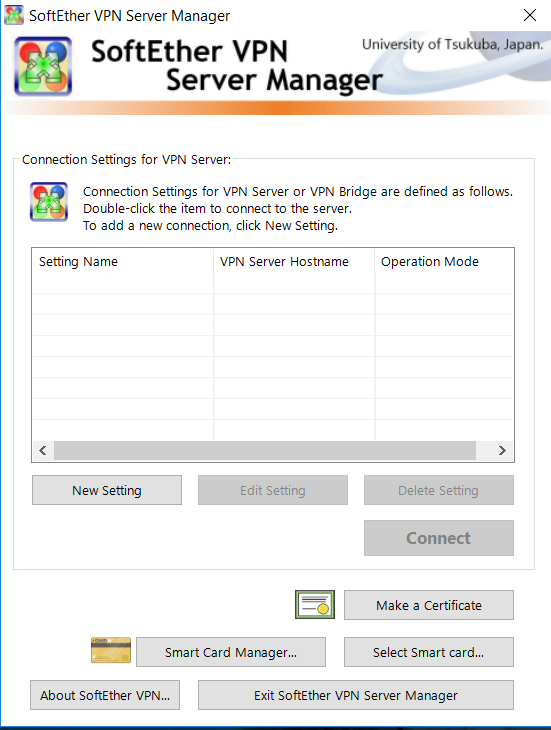
\includegraphics[width=0.6\textwidth]{SoftEther/korak8}
     \caption{Početni prozor aplikacije SoftEther}
\end{figure}
\FloatBarrier
Stvaranje servera započinje se upisom željenog naziva u polje ``setting name'' i upisom vlastite IP adrese preko koje je trenutno računalo spojeno na Internet kao što prikazano na slici \ref{fig:novaveza-soft}. Pravilan odabir ispravne IP i porta preko kojeg će se obavljati uspostava veze mora biti 
Preporuka je dodati lozinku za pristup serveru radi dodatne sigurnosti u polje ``password''.
\begin{figure}[h!]
     \centering
     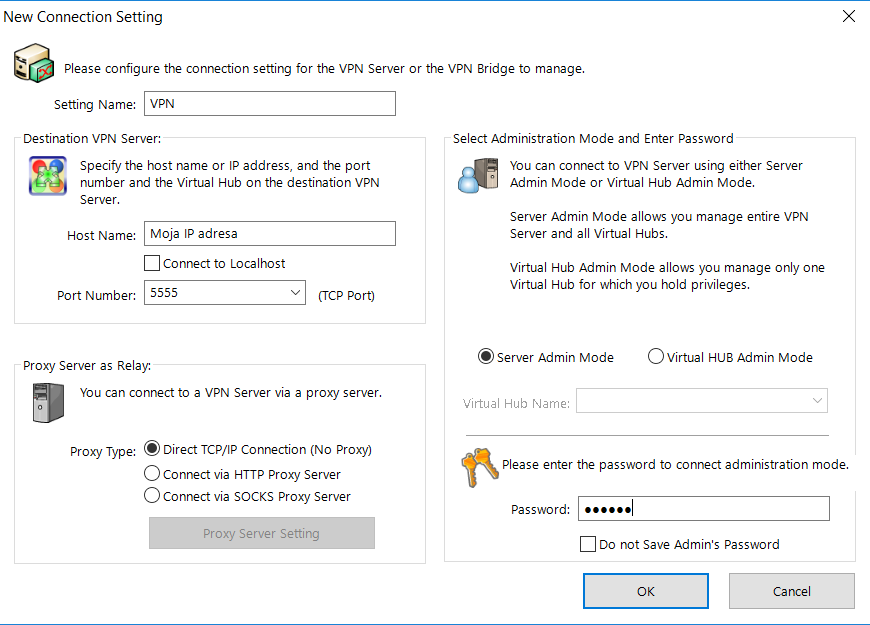
\includegraphics[width=0.8\textwidth]{SoftEther/korak9}
     \caption{Dodavanje nove veze}
     \label{fig:novaveza-soft}
\end{figure}
\FloatBarrier
U tablici je na slici \ref{fig:konf-soft}. sada vidiljiv novo dodani server kojeg je potrebno konfigurirati odabirom ``Connect'' opcije.
\begin{figure}[h!]
     \centering
     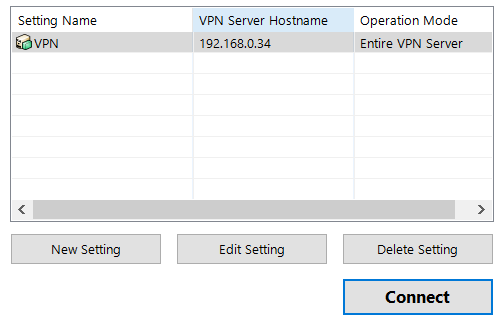
\includegraphics[width=0.6\textwidth]{SoftEther/korak10}
     \caption{Odabir konfiguracije}
     \label{fig:konf-soft}
\end{figure}
\FloatBarrier
Kako bi se druga računala uspjela povezati na stvorni virtualni server, potrebno je dodati virtualno čvorište odabirom opcije ``Create a Virtual Hub'' što je naglašeno na slici \ref{fig:mogu-soft}.
\begin{figure}[h!]
     \centering
     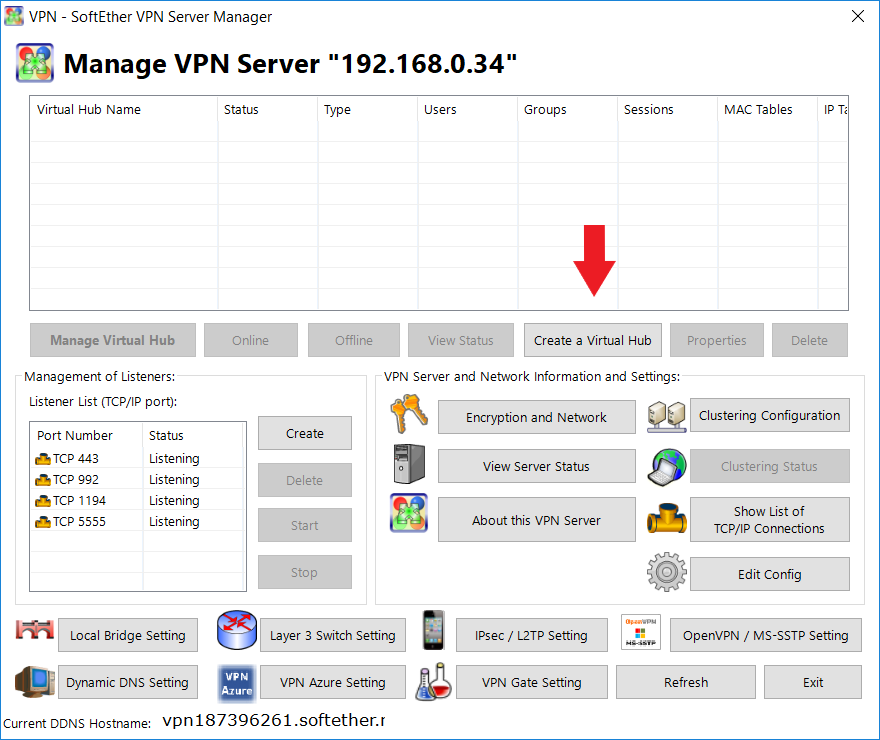
\includegraphics[width=0.6\textwidth]{SoftEther/korak11}
     \caption{Mogućnosti servera}
     \label{fig:mogu-soft}
\end{figure}
\FloatBarrier
Virtualnom čvorištu postavljamo proizvoljno ime te dodajemo lozinku radi dodatne sigurnosti.
\begin{figure}[h!]
     \centering
     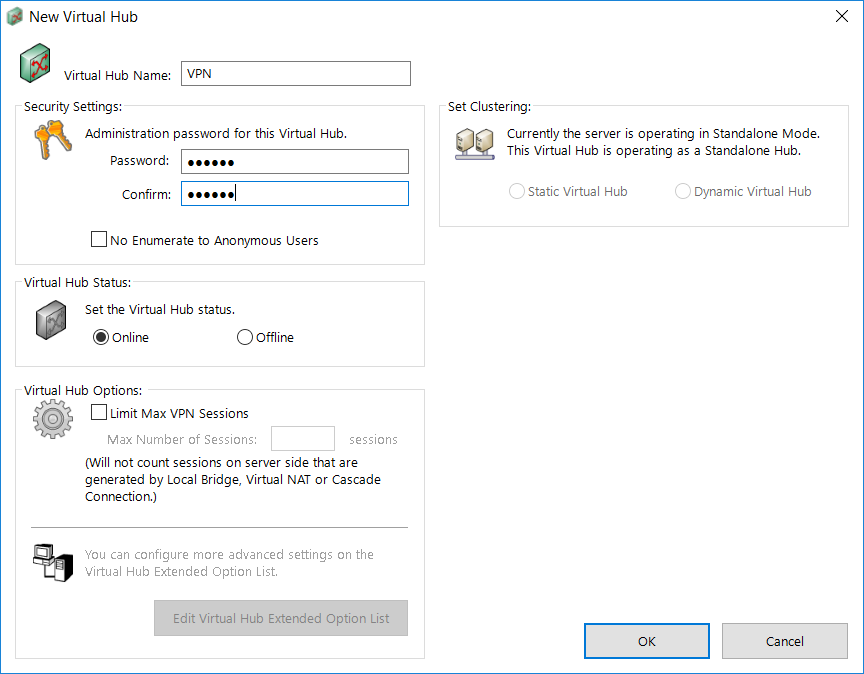
\includegraphics[width=0.6\textwidth]{SoftEther/korak12}
     \caption{Dodavanje virtualnog čvorišta}
\end{figure}
\FloatBarrier
Sada se može vidjeti novo dodano čvorište u tablici na slici \ref{fig:list-soft}.
\begin{figure}[h!]
     \centering
     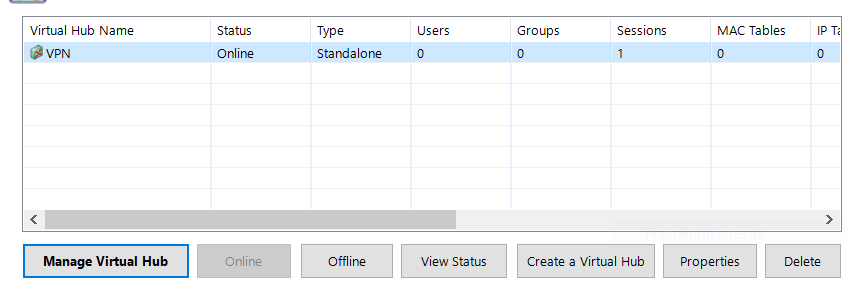
\includegraphics[width=0.8\textwidth]{SoftEther/korak13}
     \caption{Dodavanje virtualnog čvorišta}
     \label{fig:list-soft}
\end{figure}
\FloatBarrier
Sljedeći je korak odrediti tko se sve može povezati na naš server, a to se radi odabirom gumba ``Manage Virtual Hub'' kao na slici \ref{fig:list-soft} nakon čega će se otvoriti prozor sa slike \ref{fig:users-soft}.
\begin{figure}[h!]
     \centering
     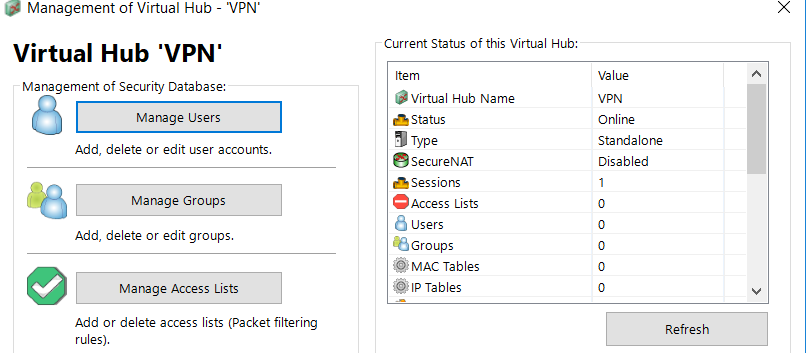
\includegraphics[width=0.7\textwidth]{SoftEther/korak14}
     \caption{Korisnici servera}
     \label{fig:users-soft}
\end{figure}
\FloatBarrier
Na prozoru sa slike \ref{fig:users-soft} odabiremo ``Manage Users''.
\begin{figure}[h!]
     \centering
     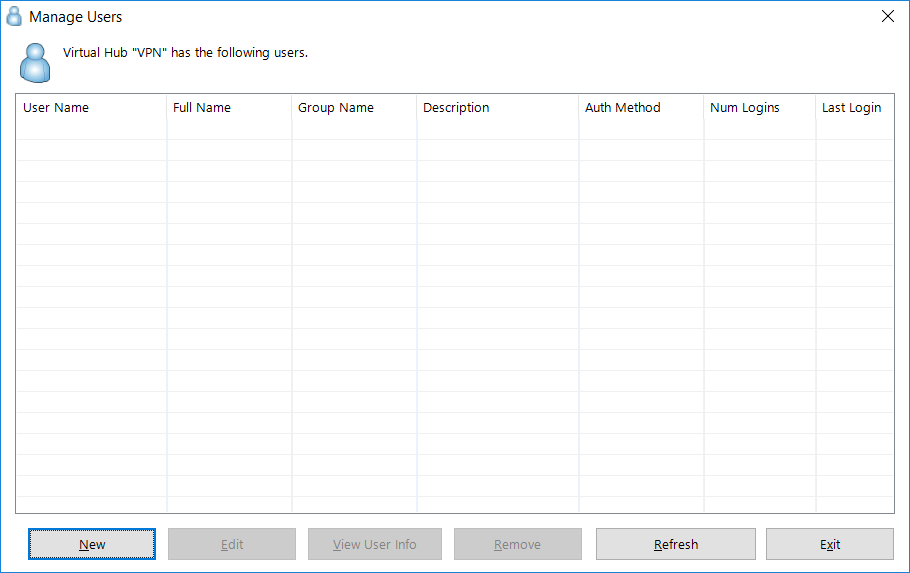
\includegraphics[width=0.5\textwidth]{SoftEther/korak15}
     \caption{Popis korisnika}
\end{figure}
\FloatBarrier
Sada dodajemo korisnika kojem ćemo dodati proizvoljno ime (u ovim je uputama korisnik nazvan ``klijent1'' i u svim narednim koracima gdje se to ime pojavljuje vama će se pojaviti vaše odabrano ime). Kako bismo smanjili vjerojatnost zlouporabe VPN-a, odabiremo mogućnost prijave klijenta uporabom našeg certifikata i lozinke. Zbog toga odabiremo ``Create Certificate'' na prozoru kao na slici \ref{fig:create-soft}.
\begin{figure}[h!]
     \centering
     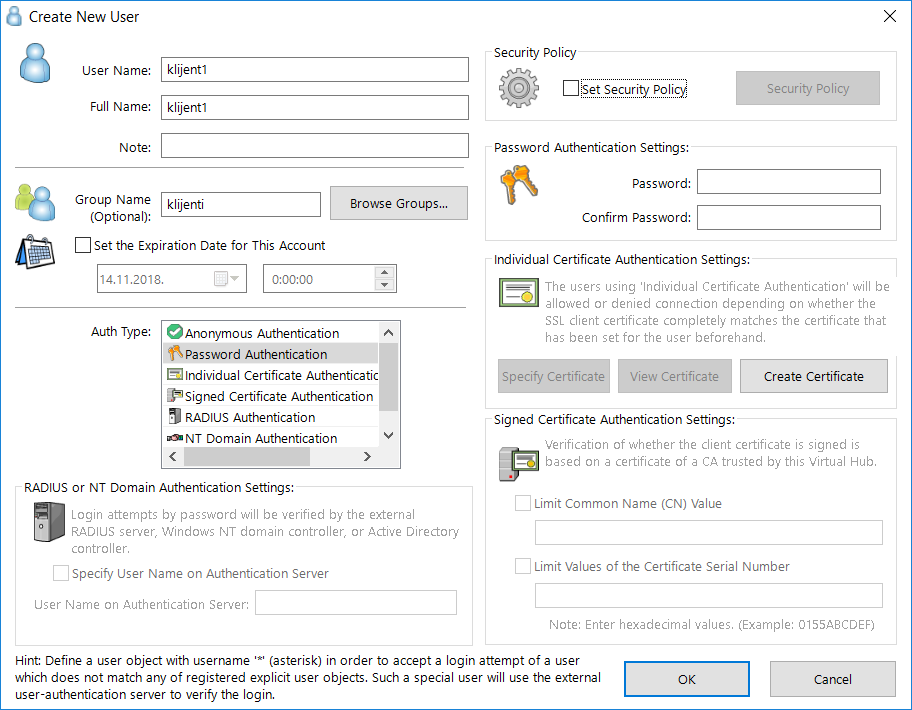
\includegraphics[width=0.8\textwidth]{SoftEther/korak16}
     \caption{Stvaranje korisnika}
     \label{fig:create-soft}
\end{figure}
\FloatBarrier
U sljedećim je poljima moguće detaljno odrediti opis stvorenog klijenta kao i vrijeme njegovog postojanja (slika \ref{fig:userca-soft}).
\begin{figure}[h!]
     \centering
     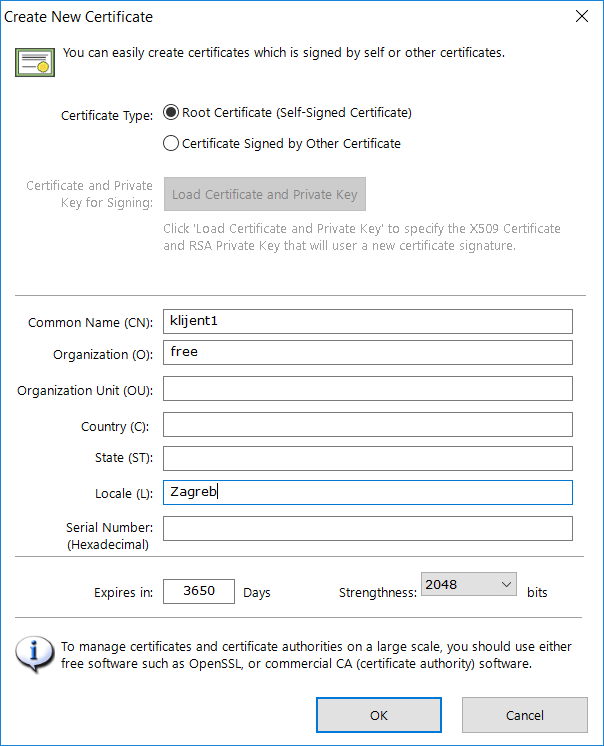
\includegraphics[width=0.6\textwidth]{SoftEther/korak17}
     \caption{Stvaranje certifikata korisnika}
     \label{fig:userca-soft}
\end{figure}
\FloatBarrier
Nakon otvaranja prozora sa slike \ref{fig:key-soft}. postavljamo lozinku kojom će se naš klijent prijavljivati na server i koja će samo njemu biti poznata.
\begin{figure}[h!]
     \centering
     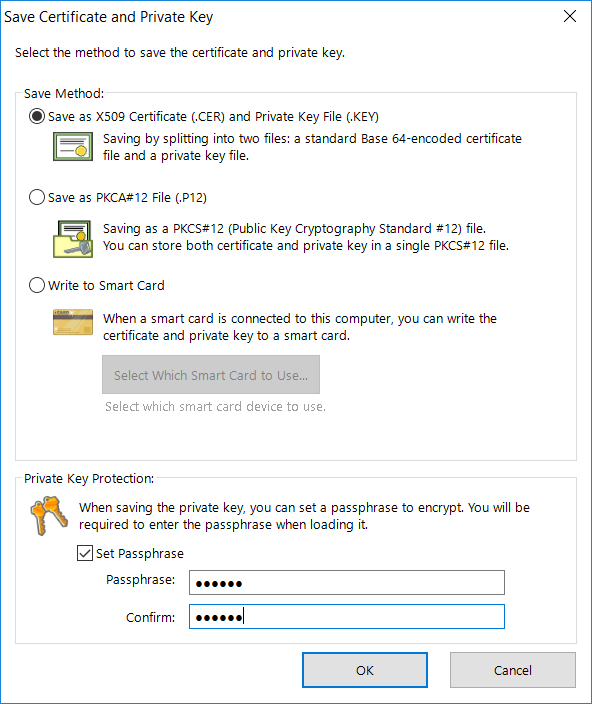
\includegraphics[width=0.6\textwidth]{SoftEther/korak18}
     \caption{Stvaranje ključa korisnika}
     \label{fig:key-soft}
\end{figure}
\FloatBarrier
Nakon potvrde nastaju dvije datoteke: jedna je .cer, a druga je .key i obje su neophodne za prijavu na naš server zato ih mi moramo spremiti i prebaciti na računala koja će se htjeti povezati na server. Povezivanje na server objašnjeno je u jednom od sljedećih dijelova poglavlja.
\begin{figure}[h!]
     \centering
     
\includegraphics[width=0.3\textwidth]{SoftEther/korak20}
     \caption{Datoteke ključ i certifikat}
\end{figure}
\FloatBarrier
Nakon potvrde vidljiv je korisnik na slici \ref{fig:new-soft} koji se može spojiti na naš server. Moguće je naravno dodavanje više različitih korisnika i brisanje istih.
\begin{figure}[h!]
     \centering
     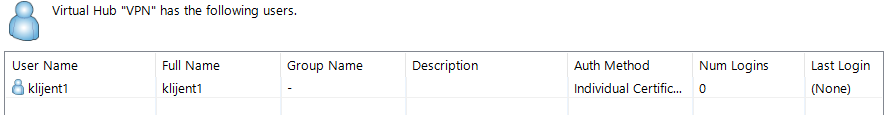
\includegraphics[width=0.9\textwidth]{SoftEther/korak19}
     \caption{Prikaz dodanog korisnika}
     \label{fig:new-soft}
\end{figure}
\FloatBarrier
%*****************************************************************
\newpage
\paragraph*{Instalacija SoftEther klijenta}

\hfill \smallbreak
Za razliku od instalacije i konfiguracije servera, instalacija je SoftEther klijenta jednostavnija. Prvi je korak preuzimanje instalacije sa službene stranice SoftEthera:\\ \url{https://www.softether.org}
\begin{figure}[h!]
	\centering
     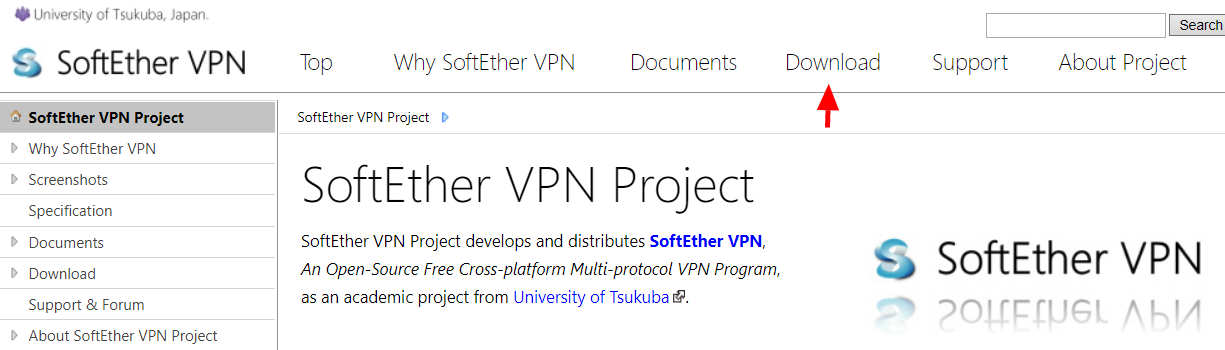
\includegraphics[width=0.75\textwidth]{SoftEther/korak1}
     	\caption{Put do instalacije}
     	\label{fig:link4-soft}
\end{figure}
\FloatBarrier
Odabirom ``Download'' iz izborne trake, što je naglašeno na slici \ref{fig:link4-soft},  prikazuje se stranica s ponuđenim poveznicama za preuzimanje od kojih se odabire ona naglašena na slici \ref{fig:link5-soft}.
\begin{figure}[h!]
     \centering
     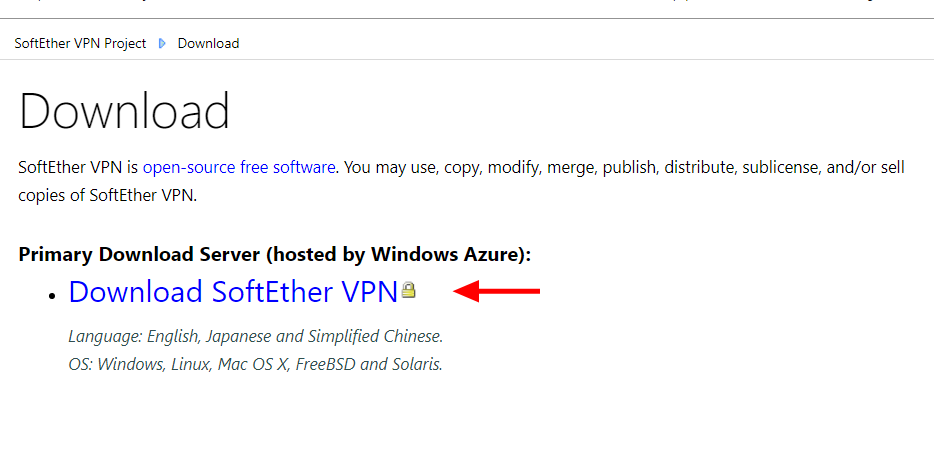
\includegraphics[width=0.65\textwidth]{SoftEther/korak2}
     \caption{Poveznica za odabir preuzimanja}
     \label{fig:link5-soft}
\end{figure}
\FloatBarrier
Sljedeći isječak (slika \ref{fig:link6-soft}) prikazuje stranicu koja se otvori odabirom prve poveznice. Na stranici se nalaze izborni okviri u kojima je potrebno odabrati željeni program. Za preuzimanje VPN klijenta potrebno je odabrati postavke prikazane na sljedećem isječku te odabrati prvu poveznicu za početak preuzimanja.
\begin{figure}[h!]
     \centering
     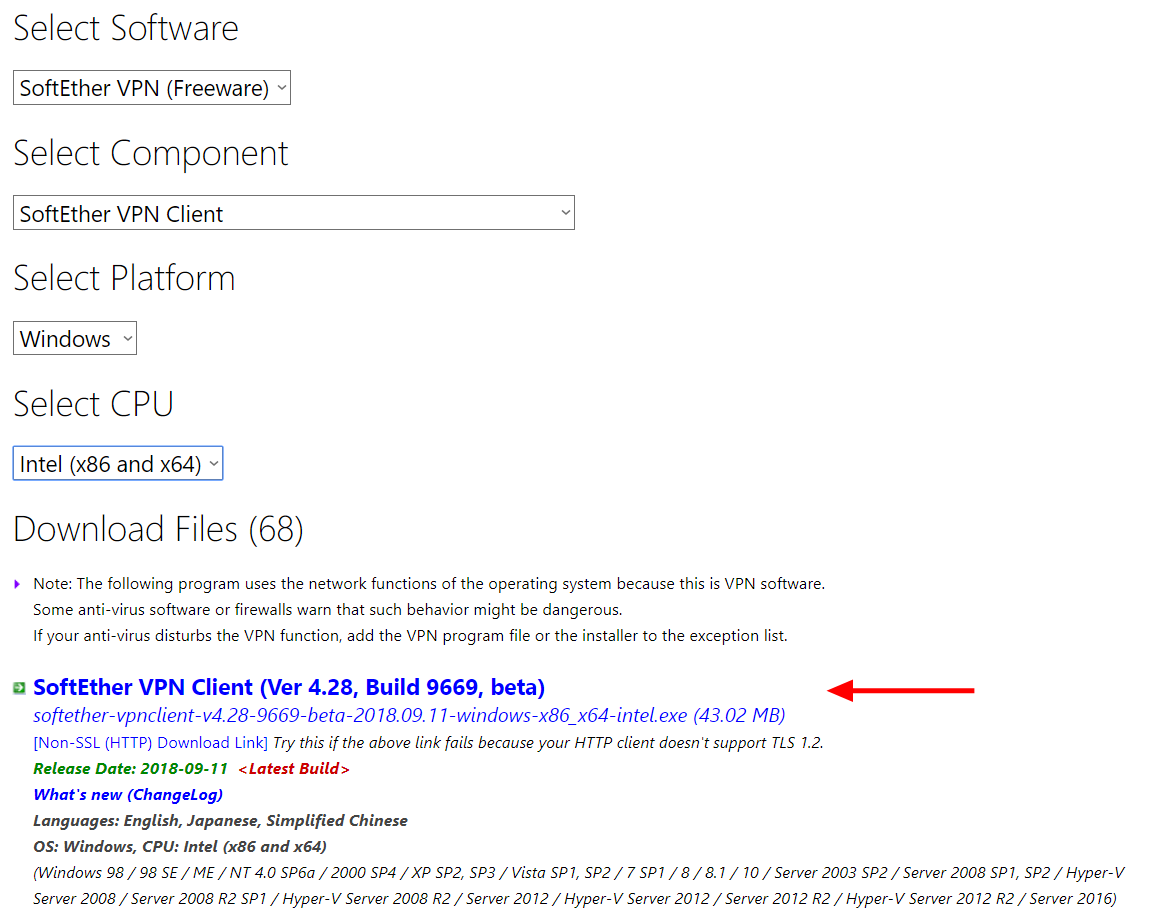
\includegraphics[width=0.75\textwidth]{SoftEther/korak3}
     \caption{Prikaz povaznice za preuzimanje}
     \label{fig:link6-soft}
\end{figure}
\FloatBarrier
Nakon završetka preuzimanja i pokretanja instalacije prikazuje se prozor kao na slici \ref{fig:odabir2-soft}. Preporuka je odabrati prvo ponuđeno jer nudi potpunu instalaciju programa.
\begin{figure}[h!]
     \centering
     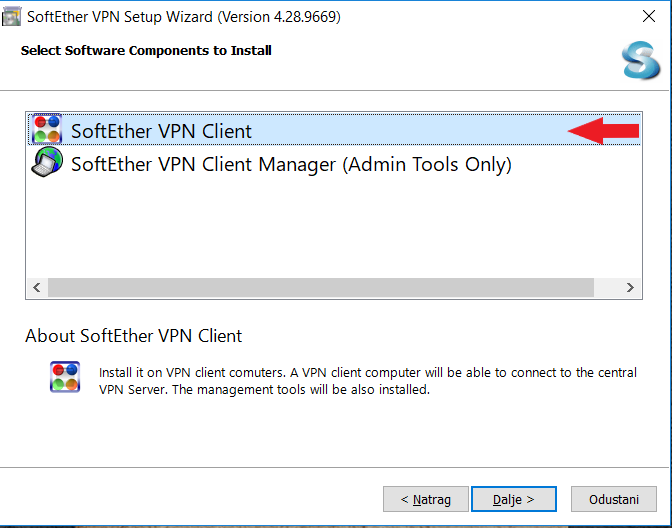
\includegraphics[width=0.6\textwidth]{SoftEther/korak4}
     \caption{Prikaz odabira klijentske instalacije}
     \label{fig:odabir2-soft}
\end{figure}
\FloatBarrier
Ukoliko je instalacija uspješno završena, prikazuje se prozor kao na slici \ref{fig:upravitelj-soft}.
\begin{figure}[h!]
     \centering
     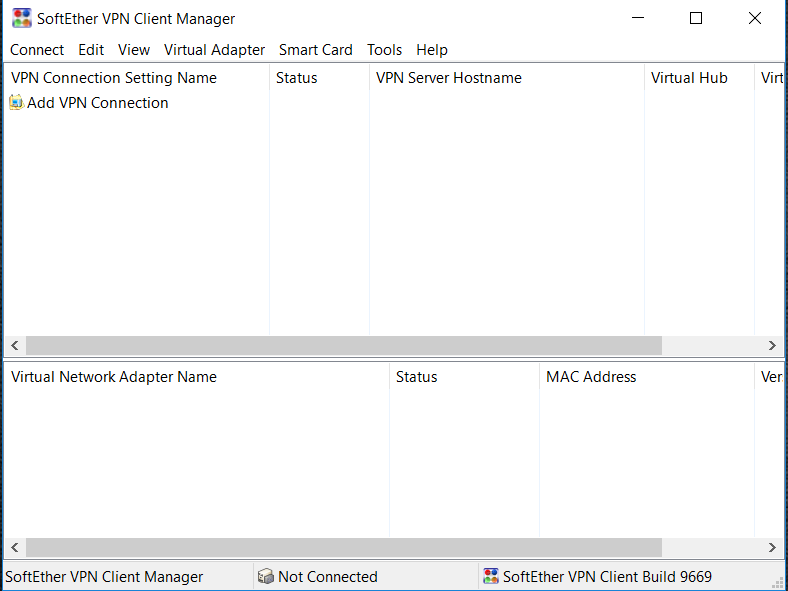
\includegraphics[width=0.7\textwidth]{SoftEther/korak5}
     \caption{Prikaz upravitelja VPN veza}
     \label{fig:upravitelj-soft}
\end{figure}
\FloatBarrier
%***********************************************************************
\newpage
\paragraph*{Povezivanje klijenta sa SoftEther serverom}

\hfill \smallbreak
Za uspješno povezivanje na stvoreni virtualni server potrebno je pokrenuti aplikaciju SoftEether VPN Client i odabrati opciju dodavanja novog VPN-a. Ako nije postavljen virtualni mrežni adapter, kao što je prikazano u sljedećem primjeru, potrebno je stvoriti novi. Prikazano je stvaranje VPN adaptera na slici \ref{fig:adapter-soft}.
\begin{figure}[h!]
     \centering
     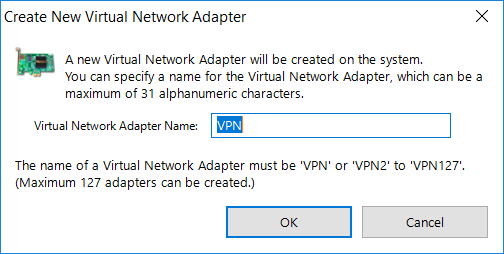
\includegraphics[width=0.6\textwidth]{SoftEther/korak21}
     \caption{Stvaranje adaptera}
     \label{fig:adapter-soft}
\end{figure}
\FloatBarrier
Nakon stvaranja adaptera moramo dodati server na koji se želimo povezati. Na slici je prikazano stvaranje veze koja se zove VPN. Slično kao i kod stvaranja servera, potrebno je upisati IP adresu preko koje se može serveru pristupiti u polje ``Host name'', tj. IP adresu nadležnog poslužitelja na kojemu je omogućeno prosljeđivanje port adresa. Aplikacija nakon upisa IP adrese dohvaća portove na koje se moguće spojiti. Izbor je nekog od ponuđenih portova proizvoljan, kao i postojećih virtualnih mrežnih adaptera. Budući da smo prilikom stvaranja korisnika servera odabrali da se on može prijaviti samo uporabom certifikata i pripadnog ključa, potrebno je stvorene datoteke ``klijent1.cer'' i ``klijent1.key'' prebaciti na računalo s kojeg se pokušava povezati na server. Učitavanje certifikata i ključa u aplikaciju obavlja se odabirom opcije ``specify client certificate'' kao u desnom dijelu slike \ref{fig:certif-soft}.
\begin{figure}[h!]
     \centering
     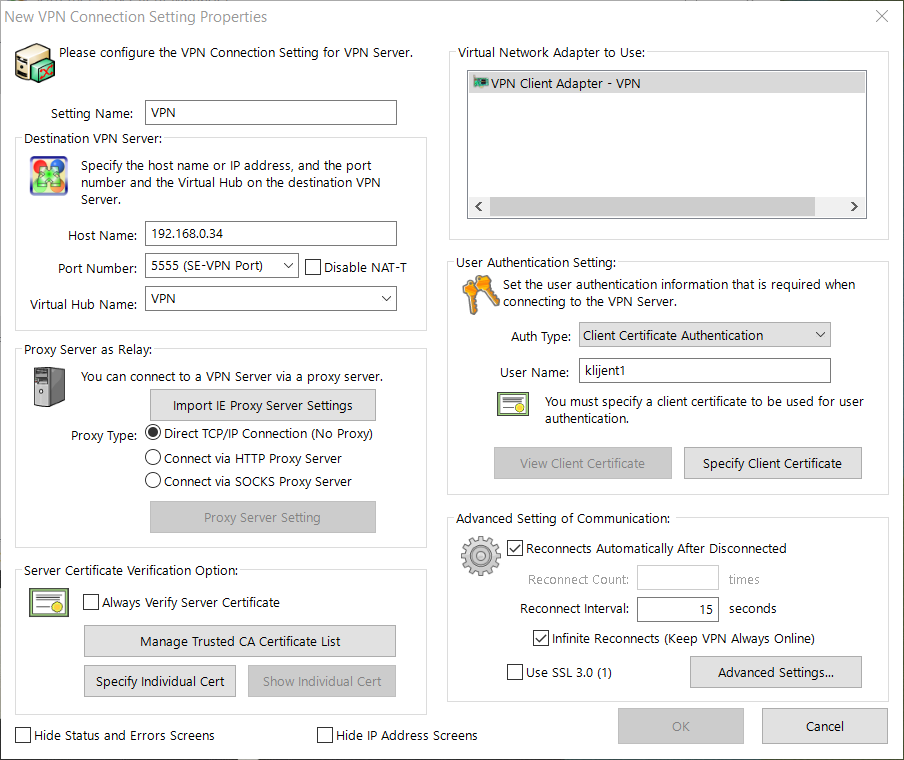
\includegraphics[width=0.8\textwidth]{SoftEther/korak22}
     \caption{Dodavanje VPN veze}
     \label{fig:certif-soft}
\end{figure}
\FloatBarrier
Nakon učitavanja datoteka prikazuje se prozor (slika \ref{fig:pass-soft}) sa sljedećeg isječka u koji se upisuje lozinka koju smo postavili prilikom stvaranja klijenta.
\begin{figure}[h!]
     \centering
     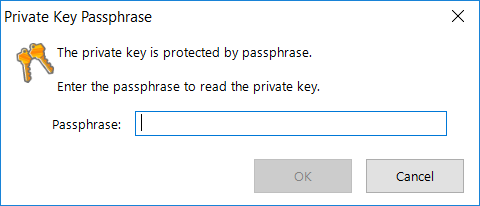
\includegraphics[width=0.6\textwidth]{SoftEther/korak23}
     \caption{Polje lozinke}
     \label{fig:pass-soft}
\end{figure}
\FloatBarrier
Ako smo učitali ispravni certifikat i unijeli ispravnu lozinku, tada će se prikazati prozor kao na slici \ref{fig:veza-soft}. na kojem vidimo povezivanje s VPN serverom.
\begin{figure}[h!]
     \centering
     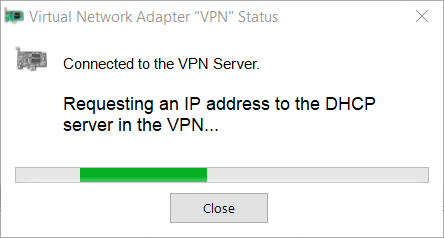
\includegraphics[width=0.5\textwidth]{SoftEther/korak24}
     \caption{Spajanje na server}
     \label{fig:veza-soft}
\end{figure}
\FloatBarrier

% pomoć pri instalaciji === https://www.youtube.com/watch?v=VbvRhPqNCsk